\documentclass{beamer}
\usepackage[utf8]{inputenc}
\usetheme{Warsaw}  %% Themenwahl
\usepackage{algpseudocode}
\usepackage{algorithm}
\usepackage{mathtools}

\title{Fehlerzustandsbaumanalyse}
\author{Öztürk Emrah, Schwartze Nicolai, Schneider Michael}
\date{\today}
\usepackage{amssymb}
\usepackage{float}

\begin{document}
\maketitle
%\frame{\tableofcontents[currentsection]}

\section{Allgemeine Informationen}
\frame{\tableofcontents[currentsection]}
\begin{frame}
	Definiertes Verfahren (EN 61025) zur Abschätzung der Ausfallswahrscheinlichkeit einer Anlage.\\~\\
	Breites Anwendungsgebiet in kritischen Branchen: Nuklearindustrie, Luft und Raumfahrt.\\~\\
	Basierend auf logischen Operationen und einfache Ausfallwahrscheinlichkeit.\\~\\
	Es existieren zwei verschiedene Verwendungsarten
	\begin{itemize}
		\item top down
		\item bottom up
	\end{itemize}
\end{frame}

\begin{frame}
\begin{figure}
	\centering
	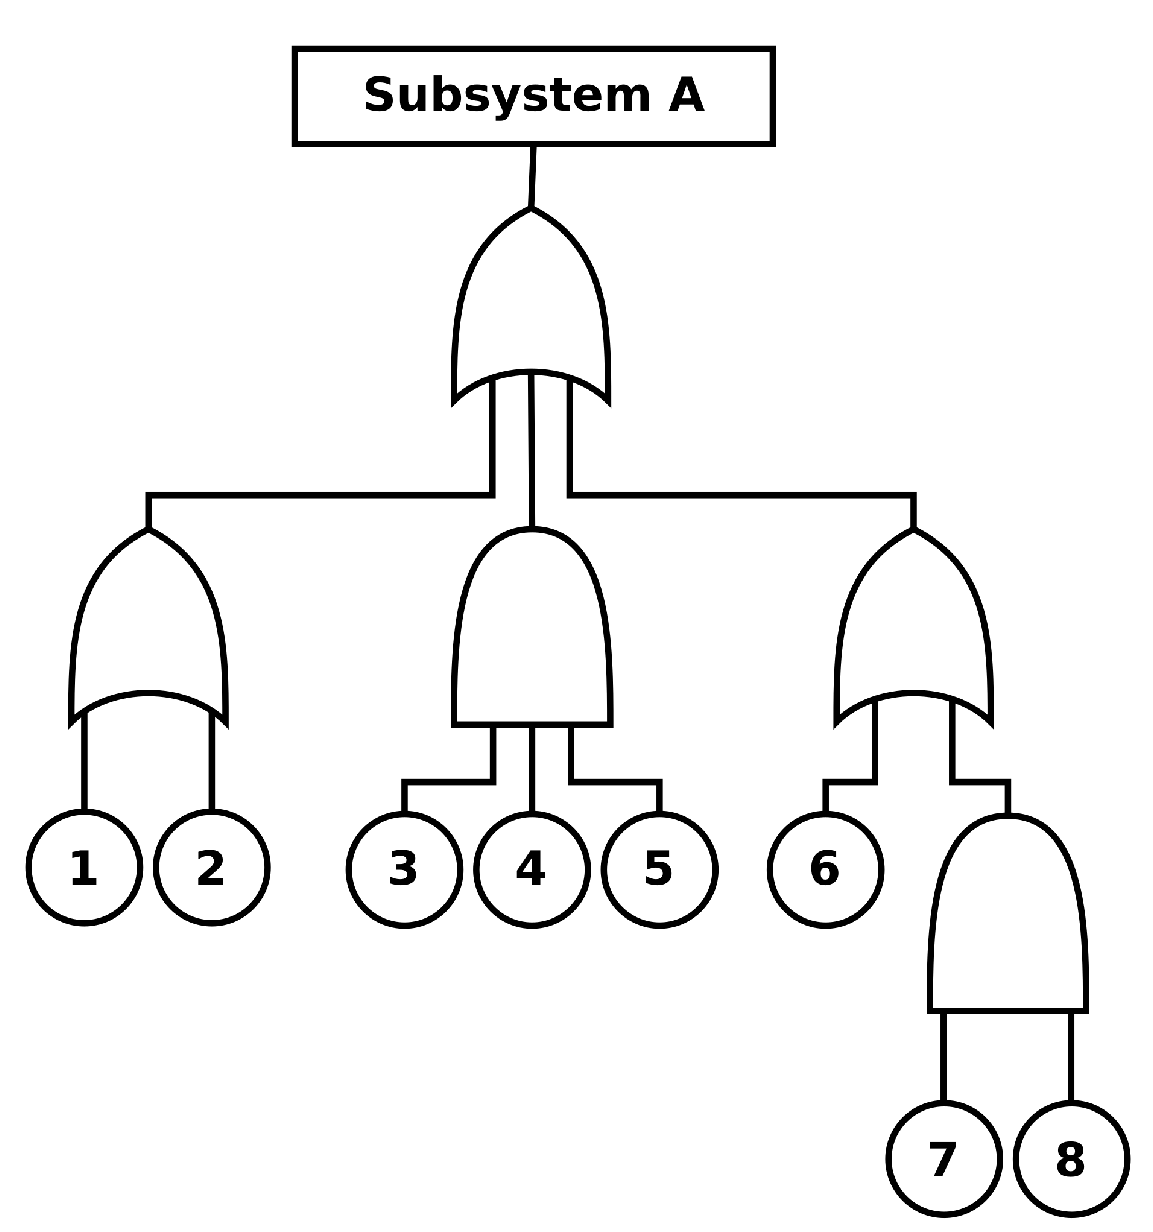
\includegraphics[width=0.6\linewidth]{fault_tree_example}
	\caption{Einfaches Fehlerzustandsbaumdiagramm Quelle: \href{https://en.wikipedia.org/wiki/Fault_tree_analysis}{https://en.wikipedia.org/wiki/Fault\textunderscore tree\textunderscore analysis}}
	\label{fig:faulttreeexample}
\end{figure}
\end{frame}

\begin{frame}
	Berechnung der Ausfallwahrscheinlichkeit mit Fehlerzustandsbaumdiagramm. 
	
	\begin{align}\label{key}
	\begin{split}
	&P(A \text{ und } B) = P(A\cap B) = P(A)P(B)\\
	&P(A \text{ oder } B) = P(A\cup B) = P(A)+P(B)-P(A)P(B)
	\end{split}
	\end{align}
\end{frame}

\section{Fehlerzustandsbaumdiagramm}
\frame{\tableofcontents[currentsection]}
\begin{frame}
	\begin{figure}[H]
		\centering
		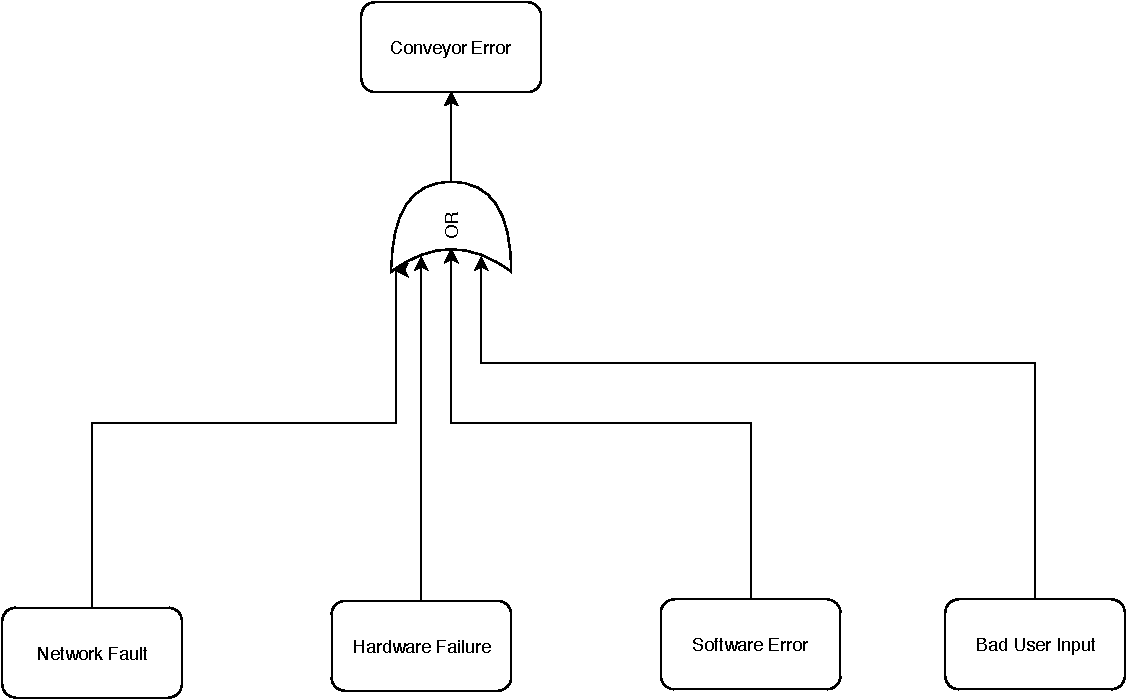
\includegraphics[width=0.7\linewidth]{../faultTreeAnalysis/FaultTreeAnalysisConveyer}
		\caption{Conveyor Error}
		\label{fig:faulttreeanalysisconveyer}
	\end{figure}
\end{frame}

\begin{frame}
	\begin{figure}[H]
		\centering
		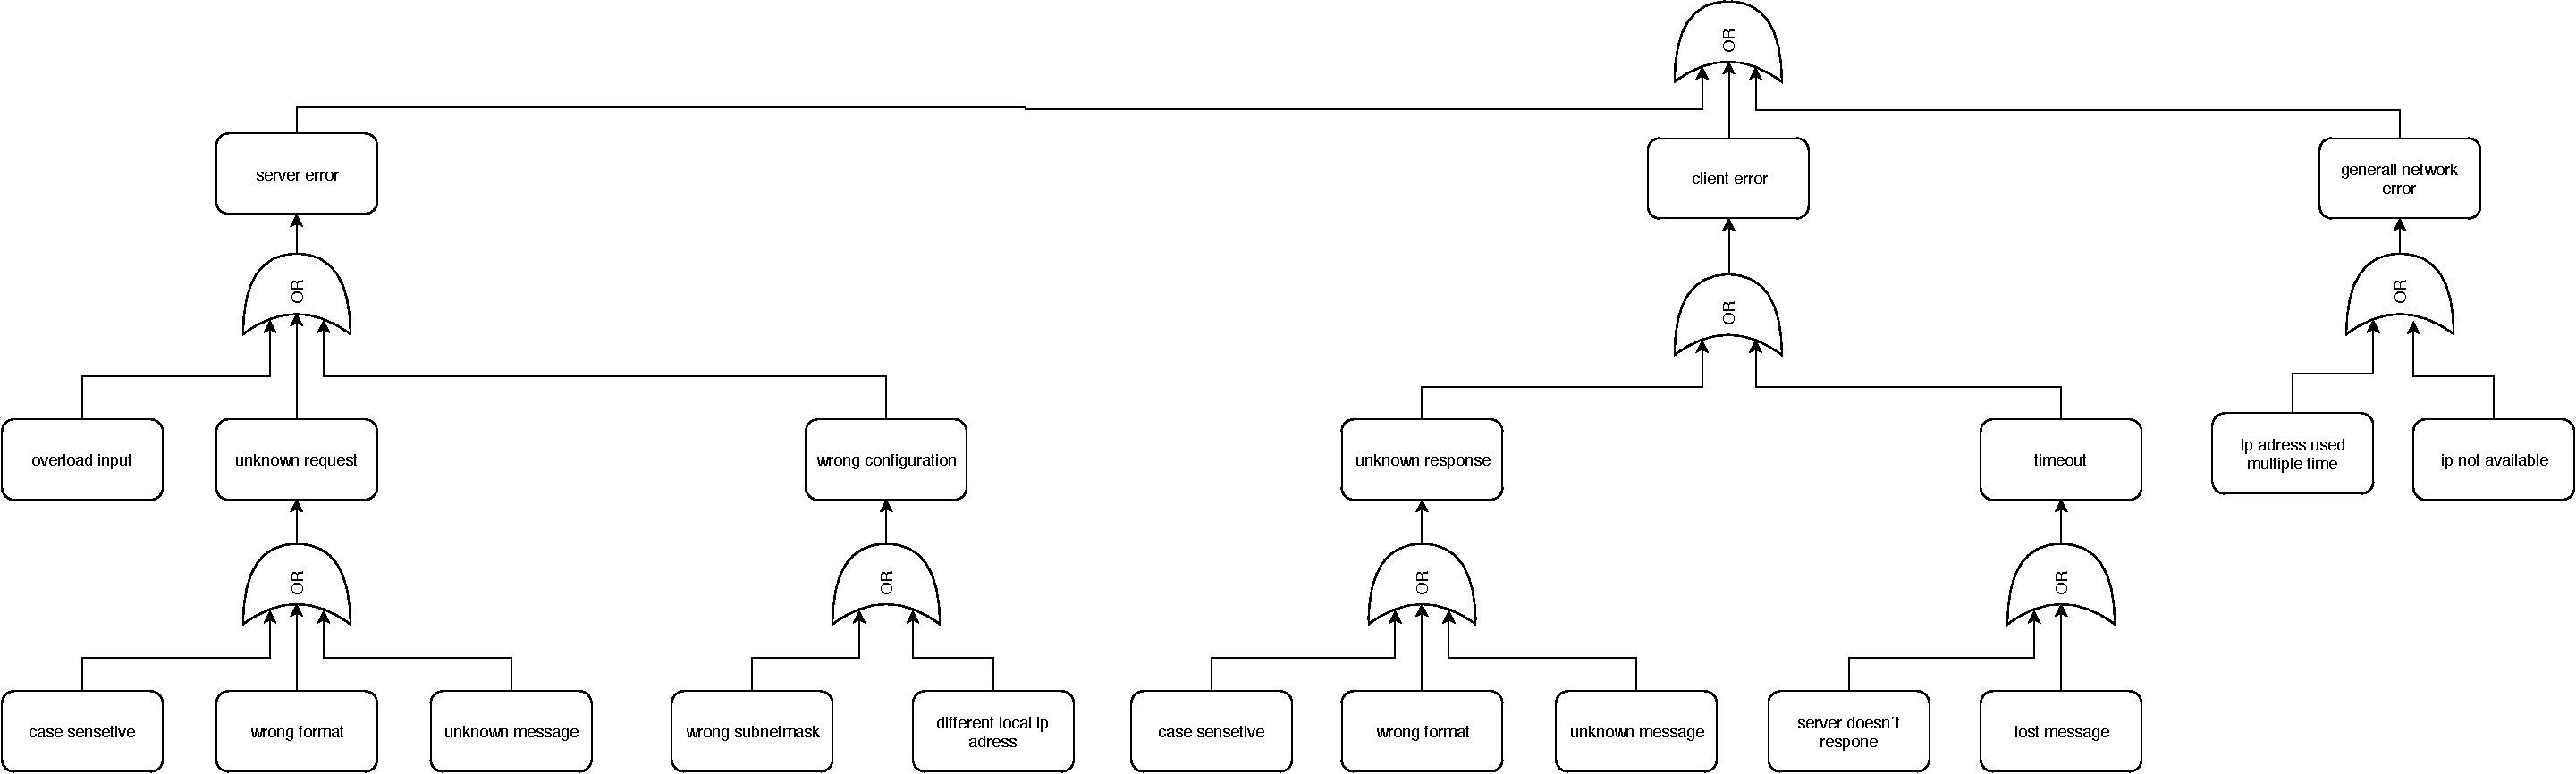
\includegraphics[width=1.05\linewidth]{../faultTreeAnalysis/FaultTreeAnalysisNetwork}
		\caption{Network Fault}
		\label{fig:faulttreeanalysisnetwork}
	\end{figure}
\end{frame}

\begin{frame}
	\begin{figure}[H]
		\centering
		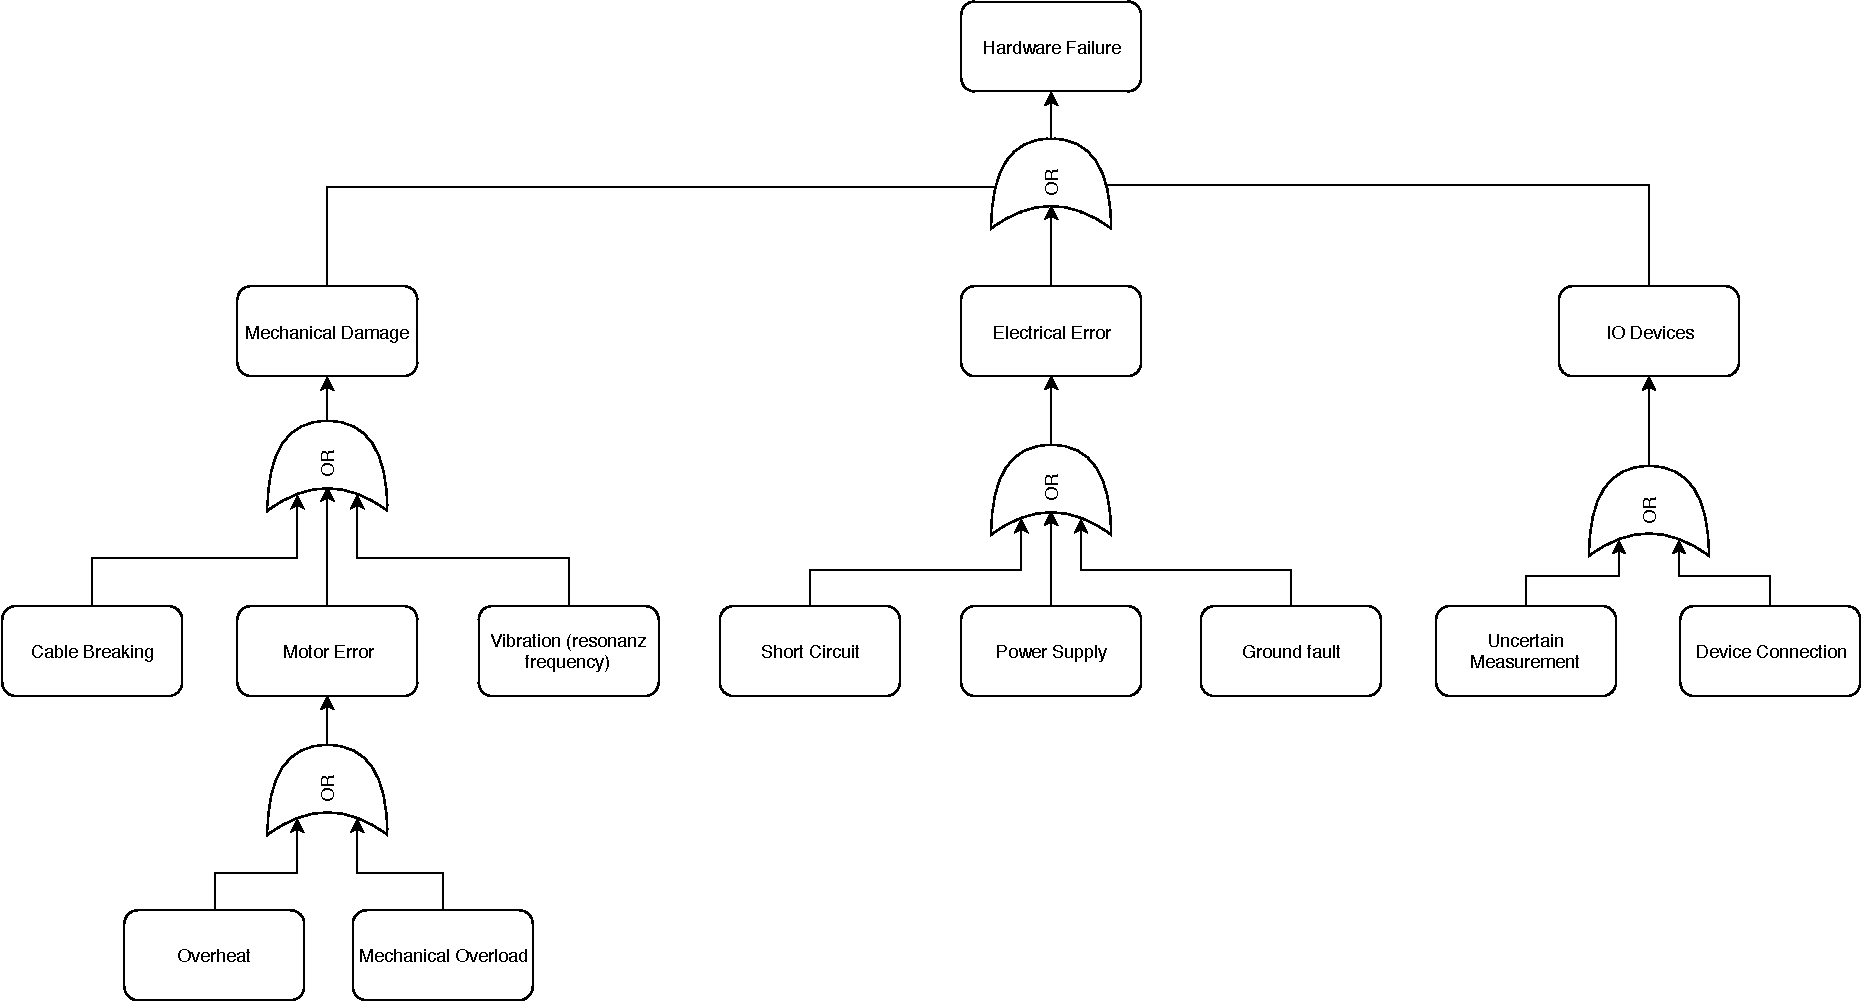
\includegraphics[width=0.9\linewidth]{../faultTreeAnalysis/FaultTreeAnalysisHardware}
		\caption{Hardware Failure}
		\label{fig:faulttreeanalysishardware}
	\end{figure}
\end{frame}

\begin{frame}
	\begin{figure}[H]
		\centering
		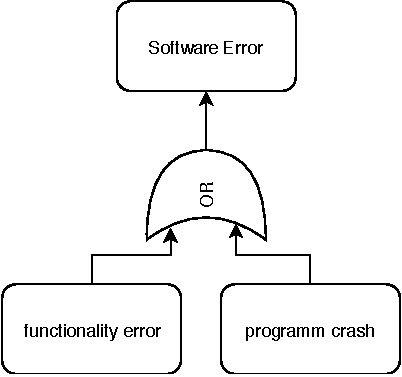
\includegraphics[width=0.4\linewidth]{../faultTreeAnalysis/FaultTreeAnalysisSoftware}
		\caption{Software Error}
		\label{fig:faulttreeanalysissoftware}
	\end{figure}
\end{frame}

\begin{frame}
	\begin{figure}[H]
		\centering
		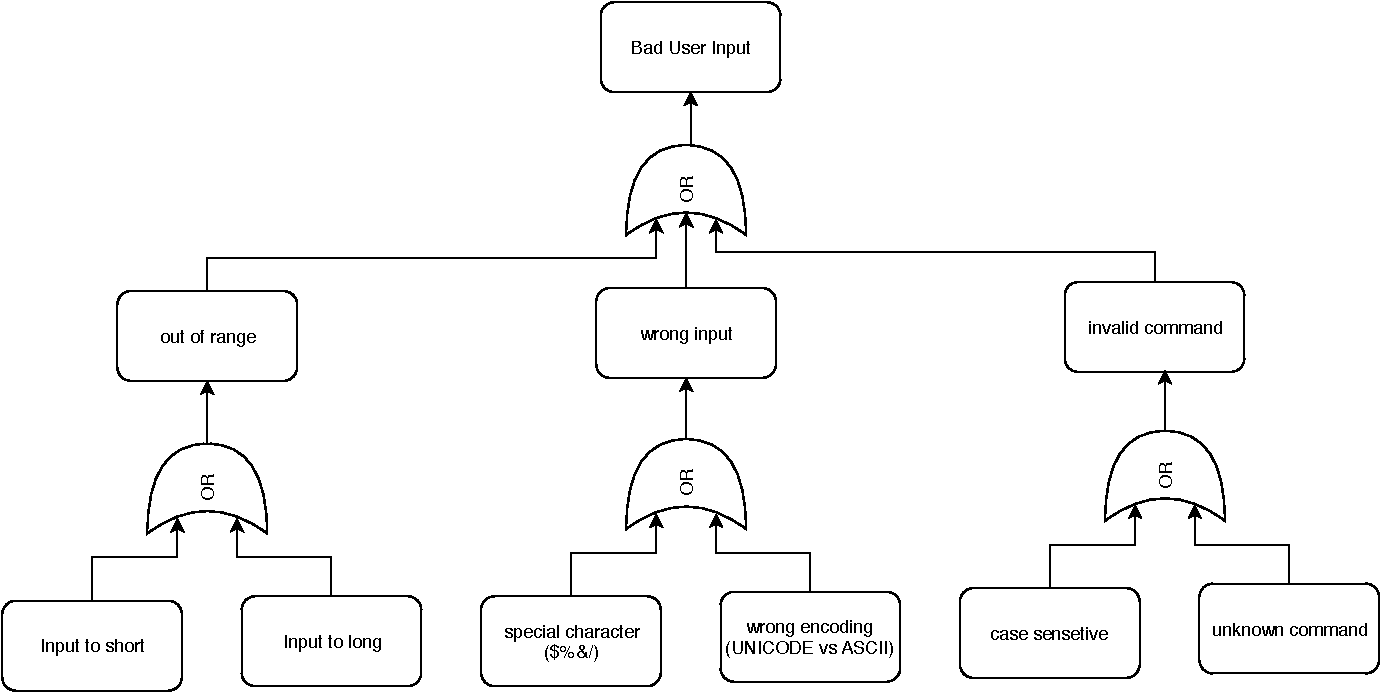
\includegraphics[width=0.8\linewidth]{../faultTreeAnalysis/FaultTreeAnalysisBadUserInput}
		\caption{Bad User Input}
		\label{fig:faulttreeanalysisbaduserinput}
	\end{figure}
	
\end{frame}
	
\section{Zusammenfassung}
\frame{\tableofcontents[currentsection]}
\begin{frame}
	Für Ermittlung der Ausfallwahrscheinlichkeit eines Systems\\~\\
	Spezielle Software erhältlich\\~\\
	Da keine einzelne Ausfallwahrscheinlichkeit vorhanden sind, konnten wir keine Berechnung durchführen.
	
	
	
	
\end{frame}

\end{document}